\section{Jointly learning syntactic parsing and semantic composition}


\subsection{Why joint learning?}

Sentence embedding methods like LSTMs and tree-structured RNNs have have rapidly become a standard tool in natural language processing tasks involving sentence meaning (TODO: Cite). These methods are generally built up out of standard neural network components, making it possible to learn them with minimal domain knowledge. They are also generally compositional, in that they build up their representations incrementally in a way that involves creating explicit representations for pieces of sentences. There is not yet any single model that is known to produce high-quality representations across domains, and one of the major open issues in the development of these models is the degree to which syntactic tree structures provide them with usable information that could not be efficiently extracted without them.

Our hypothesis on this issue is in two parts. (i) As is near-universally accepted in the language sciences, central components of natural language meaning are constructed compositionally according to regular tree structures in which each node in the tree structure for a sentence has an interpretable meaning derivable from the meanings of its children. Representation learning systems can learn more effectively by taking advantage of this fact. (ii) The syntactic structures used by typical software parsers do not reliably match the true tree structures underlying the construction of meaning for several reasons, even when those parsers are functioning correctly. In light of these two points, we propose a class of models which simultaneously learn to parse natural language sentences and to create compositional semantic representations using those parse structures, and can do this using supervision from both a downstream semantic task like sentiment classification and, when appropriate a syntactic parser. Such a model then serve both as a parser which is tuned so as to be optimally supportive of the construction of sentence meaning, as a function to construct representations of sentence meaning.


\begin{figure}[tp]
  \centering\small
 	 \begin{tikzpicture}
    \def\dx{18pt}
    \def\dy{30pt}
    \newcounter{i}
    \tikzstyle{highlight}=[fill=black!10]
    \tikzstyle{comment}=[color=blue!80!black]
    
    \stepcounter{i}\node  (\arabic{i}) at (0*\dx,6*\dy) {$\vec{y}^{(1, 1)}$};
    \stepcounter{i}\node  (\arabic{i}) at (-1*\dx,5*\dy) {$\vec{y}^{(2, 1)}$};
    \stepcounter{i}\node  (\arabic{i}) at (1*\dx,5*\dy) {$\vec{y}^{(2, 2)}$};
    \stepcounter{i}\node  (\arabic{i}) at (-2*\dx,4*\dy) {$\vec{y}^{(3, 1)}$};
    \stepcounter{i}\node  (\arabic{i}) at (0*\dx,4*\dy) {$\vec{y}^{(3, 2)}$};
    \stepcounter{i}\node[highlight]  (\arabic{i}) at (2*\dx,4*\dy) {$\vec{y}^{(3, 3)}$};
    \stepcounter{i}\node[highlight]  (\arabic{i}) at (-3*\dx,3*\dy) {$\vec{y}^{(4, 1)}$};
    \stepcounter{i}\node  (\arabic{i}) at (-1*\dx,3*\dy) {$\vec{y}^{(4, 2)}$};
    \stepcounter{i}\node  (\arabic{i}) at (1*\dx,3*\dy) {$\vec{y}^{(4, 3)}$};
    \stepcounter{i}\node  (\arabic{i}) at (3*\dx,3*\dy) {$\vec{y}^{(4, 4)}$};
    \stepcounter{i}\node  (\arabic{i}) at (-4*\dx,2*\dy) {$\vec{y}^{(5, 1)}$};
    \stepcounter{i}\node  (\arabic{i}) at (-2*\dx,2*\dy) {$\vec{y}^{(5, 2)}$};
    \stepcounter{i}\node  (\arabic{i}) at (0*\dx,2*\dy) {$\vec{y}^{(5, 3)}$};
    \stepcounter{i}\node  (\arabic{i}) at (2*\dx,2*\dy) {$\vec{y}^{(5, 4)}$};
    \stepcounter{i}\node[highlight]  (\arabic{i}) at (4*\dx,2*\dy) {$\vec{y}^{(5, 5)}$};
    \stepcounter{i}\node  (\arabic{i}) at (-5*\dx,1*\dy) {My};
    \stepcounter{i}\node  (\arabic{i}) at (-3*\dx,1*\dy) {hovercraft};
    \stepcounter{i}\node  (\arabic{i}) at (-1*\dx,1*\dy) {is};
    \stepcounter{i}\node  (\arabic{i}) at (1*\dx,1*\dy) {full};
    \stepcounter{i}\node  (\arabic{i}) at (3*\dx,1*\dy) {of};
    \stepcounter{i}\node  (\arabic{i}) at (5*\dx,1*\dy) {eels};
   
    \stepcounter{i}\node[comment]  (\arabic{i}) at (4*\dx,4*\dy) {\textsc{compose}};
    \stepcounter{i}\node[comment]  (\arabic{i}) at (-5*\dx,3*\dy) {\textsc{copy-L}};
    \stepcounter{i}\node[comment]  (\arabic{i}) at (6*\dx,2*\dy) {\textsc{copy-R}};
   
    \tikzstyle{extra} = [->, draw=black!50, line width=0.8pt]
    \tikzstyle{valid} = [->, draw=black, line width=1.4pt]

          \draw [valid] (2) -- (1);
          \draw [valid] (3) -- (1);
          
          \draw [valid] (4) -- (2);
          \draw [extra] (5) -- (2);
          \draw [valid] (5) -- (3);
          \draw [valid] (6) -- (3);
          
          \draw [valid] (7) -- (4);
          \draw [extra] (8) -- (4);
          \draw [valid] (8) -- (5);
          \draw [extra] (9) -- (5);
          \draw [valid] (9) -- (6);
          \draw [valid] (10) -- (6);
          
          \draw [valid] (11) -- (7);
          \draw [extra] (12) -- (7);
          \draw [valid] (12) -- (8);
          \draw [extra] (13) -- (8);
          \draw [valid] (13) -- (9);
          \draw [extra] (14) -- (9);
          \draw [valid] (14) -- (10);
          \draw [valid] (15) -- (10);
          
          \draw [valid] (16) -- (11);
          \draw [valid] (17) -- (11);
          \draw [extra] (17) -- (12);
          \draw [valid] (18) -- (12);
          \draw [extra] (18) -- (13);
          \draw [valid] (19) -- (13);
          \draw [extra] (19) -- (14);
          \draw [valid] (20) -- (14);
          \draw [extra] (20) -- (15);
          \draw [valid] (21) -- (15);
  \end{tikzpicture}

        \caption{The connection structure of a LatticeNN. The correct binary parse tree for the example sentence, projected onto a lattice with the left-first rule, is shown in the bolded arrows.}
  \label{lattice-fig1}
\end{figure}


If our hypothesis is correct, and our models succeed at their goals, two important objectives will be served. The first is an engineering objective: our sentence embedding model will exploit compositional structure in the most effective way possible, producing better sentence representations that would have been possible otherwise. The second is a scientific objective: by learning a syntax optimal for semantic composition, we have a new source of information about humans might take advantage of syntactic structure in understanding natural language. This research is becoming possible only now, as it depends on both the tools (both software and hardware) for effectively training large neural networks that are only now becoming available, as well as on the availability of large volumes of natural language sentences annotated with explicit information about sentence meaning that are only now being collected.

\paragraph{What's wrong with existing parsers?} One source of error is obvious: the parsers that are typically used to generate constituency or dependency structures for sentences are built around statistical machine learning systems trained on data that reflects only a fraction of the massive diversity of natural language, and a certain amount of error from both underfitting and overfitting is essentially unavoidable in this context. This is not, at least primarily, the kind of error that we aim to avoid. Our interest is in two other sources of error: cases of \textbf{syntax-semantics mismatch} where even the correct syntactic parse under the relevant formalism does not express the way in which meanings are constructed, and cases of \textbf{syntactic ambiguity} where there are multiple syntactically correct tree structures, and where choosing only one of them would mask a genuine ambiguity in meaning.

% TODO: Example constructions for each!

\subsection{Parsing in lattices} 

In this section, we propose a simple framework for syntactic parsing that lends itself joint learning. It is centered around a triangular lattice structure of the kind shown in Fig.~\ref{lattice-fig1}. In the lattice, every node in the bottom row contains a vector representation for a single word, the top node contains a vector representation of the whole sentence (of the same dimension), and every intermediate node contains a vector representation of some subset of the sentence.

\begin{figure}[tp]
  \centering\small
 	 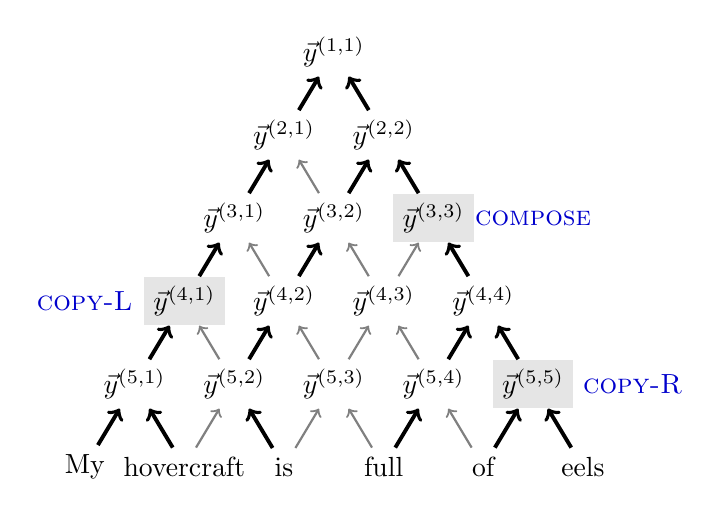
\begin{tikzpicture}{
    \def\dx{18pt}
    \def\dy{30pt}
    \newcounter{i-b}
    \tikzstyle{highlight}=[fill=black!10]
    \tikzstyle{comment}=[color=blue!80!black]
    
    \stepcounter{i-b}\node  (\arabic{i-b}) at (0*\dx,6*\dy) {$\vec{y}^{(1, 1)}$};
    \stepcounter{i-b}\node  (\arabic{i-b}) at (-1*\dx,5*\dy) {$\vec{y}^{(2, 1)}$};
    \stepcounter{i-b}\node  (\arabic{i-b}) at (1*\dx,5*\dy) {$\vec{y}^{(2, 2)}$};
    \stepcounter{i-b}\node  (\arabic{i-b}) at (-2*\dx,4*\dy) {$\vec{y}^{(3, 1)}$};
    \stepcounter{i-b}\node  (\arabic{i-b}) at (0*\dx,4*\dy) {$\vec{y}^{(3, 2)}$};
    \stepcounter{i-b}\node[highlight]  (\arabic{i-b}) at (2*\dx,4*\dy) {$\vec{y}^{(3, 3)}$};
    \stepcounter{i-b}\node[highlight]  (\arabic{i-b}) at (-3*\dx,3*\dy) {$\vec{y}^{(4, 1)}$};
    \stepcounter{i-b}\node  (\arabic{i-b}) at (-1*\dx,3*\dy) {$\vec{y}^{(4, 2)}$};
    \stepcounter{i-b}\node  (\arabic{i-b}) at (1*\dx,3*\dy) {$\vec{y}^{(4, 3)}$};
    \stepcounter{i-b}\node  (\arabic{i-b}) at (3*\dx,3*\dy) {$\vec{y}^{(4, 4)}$};
    \stepcounter{i-b}\node  (\arabic{i-b}) at (-4*\dx,2*\dy) {$\vec{y}^{(5, 1)}$};
    \stepcounter{i-b}\node  (\arabic{i-b}) at (-2*\dx,2*\dy) {$\vec{y}^{(5, 2)}$};
    \stepcounter{i-b}\node  (\arabic{i-b}) at (0*\dx,2*\dy) {$\vec{y}^{(5, 3)}$};
    \stepcounter{i-b}\node  (\arabic{i-b}) at (2*\dx,2*\dy) {$\vec{y}^{(5, 4)}$};
    \stepcounter{i-b}\node[highlight]  (\arabic{i-b}) at (4*\dx,2*\dy) {$\vec{y}^{(5, 5)}$};
    \stepcounter{i-b}\node  (\arabic{i-b}) at (-5*\dx,1*\dy) {My};
    \stepcounter{i-b}\node  (\arabic{i-b}) at (-3*\dx,1*\dy) {hovercraft};
    \stepcounter{i-b}\node  (\arabic{i-b}) at (-1*\dx,1*\dy) {is};
    \stepcounter{i-b}\node  (\arabic{i-b}) at (1*\dx,1*\dy) {full};
    \stepcounter{i-b}\node  (\arabic{i-b}) at (3*\dx,1*\dy) {of};
    \stepcounter{i-b}\node  (\arabic{i-b}) at (5*\dx,1*\dy) {eels};
   
    \stepcounter{i-b}\node[comment]  (\arabic{i-b}) at (4*\dx,4*\dy) {\textsc{compose}};
    \stepcounter{i-b}\node[comment]  (\arabic{i-b}) at (-5*\dx,3*\dy) {\textsc{copy-L}};
    \stepcounter{i-b}\node[comment]  (\arabic{i-b}) at (6*\dx,2*\dy) {\textsc{copy-R}};
   
    \tikzstyle{extra} = [->, draw=black!50, line width=0.8pt]
    \tikzstyle{valid} = [->, draw=black, line width=1.4pt]

          \draw [valid] (2) -- (1);
          \draw [valid] (3) -- (1);
          
          \draw [valid] (4) -- (2);
          \draw [extra] (5) -- (2);
          \draw [valid] (5) -- (3);
          \draw [valid] (6) -- (3);
          
          \draw [valid] (7) -- (4);
          \draw [extra] (8) -- (4);
          \draw [valid] (8) -- (5);
          \draw [extra] (9) -- (5);
          \draw [extra] (9) -- (6);
          \draw [valid] (10) -- (6);
          
          \draw [valid] (11) -- (7);
          \draw [extra] (12) -- (7);
          \draw [valid] (12) -- (8);
          \draw [extra] (13) -- (8);
          \draw [extra] (13) -- (9);
          \draw [extra] (14) -- (9);
          \draw [valid] (14) -- (10);
          \draw [valid] (15) -- (10);
          
          \draw [valid] (16) -- (11);
          \draw [valid] (17) -- (11);
          \draw [extra] (17) -- (12);
          \draw [valid] (18) -- (12);
          \draw [extra] (18) -- (13);
          \draw [extra] (19) -- (13);
          \draw [valid] (19) -- (14);
          \draw [extra] (20) -- (14);
          \draw [valid] (20) -- (15);
          \draw [valid] (21) -- (15);}
  \end{tikzpicture}

        \caption{The correct binary parse tree for the example sentence, projected onto a lattice \textit{without} the left-first rule.}
  \label{lattice-fig1}
\end{figure}



\subsection{Model definition}

To compute the vector representation for a sentence, we populate the bottom row of the structure $\vec{y}^{(N,1...N)}$ with the embedddings of each of the words. We then compute the representations of each row starting at the second row from the bottom ($N - 1$), and moving from left to right. Computing one feature vector requires two stages. In the first step, we produce a distribution $\vec{o}$ over the operations \{\textsc{copy-L, copy-R, compose}\}, and in the second step, that distribution is used to compute a feature vector $\vec{y}$.

At each row $i$, we begin by computing a scoring feature vector $\vec{s}$ for each node $(i, j)$ which is meant to contain features that allow the model to judge how appropriate it would be to compose the two child nodes $(i+1, j)$ and $(i+1, j+1)$ at $(i, j)$. This decision is made primarily on the basis of the two child nodes, and a $C$-word window of context around them that is meant to allow the model to do a limited amount of ambiguity resolution. When the context window extends off the edge of the lattice in either direction, a single learned padding vector is used. % TODO
Including $\frac{j}{i}$ and $j$ as additional features here is intended to allow the model to learn to use linear order in making its scoring decisions, allowing it to prefer to compose pairs of constituens that are closer to the left edge of the tree when all else is equal, and encouraging the model to conform to our left-first rule.

\begin{equation}
\label{scoringeqn}
\vec{s}^{(i,j)} = \tanh(\mathbf{M}_s \colvec{8}
	{\vec{y}^{(i + 1, j - C + 1)}}
	{...}
	{\vec{y}^{(i + 1, j)}}
	{\vec{y}^{(i + 1, j + 1)}}
	{...}
	{\vec{y}^{(i + 1, j + C)}}
	{\frac{j}{i}}
	{j}
	  + \vec{b_s}) \\
\end{equation}
%
To convert these feature vectors to single scores, we take their inner product with a parameter vector $\vec{v}^T_s$. Since we wish for the model to compose only one pair of child nodes at each row $i$, we apply a softmax function to the full vector of scores computed at each row, and use the resulting values (which sum to one) to decide which nodes to compose.
%
\begin{equation} 
o^{(i,\,...)}_{\textsc{compose}} = \text{softmax}(\colvec{4}
	{\vec{v}^T_s \vec{s}^{(i, 1)} }
	{\vec{v}^T_s \vec{s}^{(i, 2)}}
	{...}
	{\vec{v}^T_s \vec{s}^{(i, i)}}	
	) \\
\end{equation}
%
At training time, optional secondary parsing supervision can be used in the form of a label $\kappa^{(i)}$ indicating the location of the merge at layer $i$ of the left-first projection of the reference parse.

Then, for each node in the current row, we use these modified scores to compute another set of values summing to one, this time representing the fraction of the activation of the current node that should be drawn from each of the three operations:
%
\begin{gather}
o^{(i, j)}_{\textsc{copy-L}} = \sum_{x = j + 1}^{i} o^{(i,x)}_{\textsc{compose}} \\
o^{(i, j)}_{\textsc{copy-R}} = \sum_{x = 1}^{j - 1} o^{(i,x)}_{\textsc{compose}}
\end{gather}
%
The use of the sum for the two \textsc{copy} weights reflects the intuition that if a pair of nodes will be composed to the left of the current node, the current node must \textsc{copy-R}, and vice versa, in order to preserve the left-first tree projection structure. 

% TODO: What guarantees can we make about how much of the activation from each layer will be propagated to the next layer?

Finally, using these three computed weights, we compute the activations for the current node, using a standard RNN activation function for the \textsc{compose} operation:
% 
\begin{equation}
\vec{h}^{(i, j)} = \tanh(\mathbf{M_y} \colvec{2}{\vec{y}^{(i + 1, j)}}{\vec{y}^{(i + 1, j + 1)}} + \vec{b}_y)
\end{equation}

\begin{eqnarray}
\vec{y}^{(i,j)} & = & o^{(i, j)}_{\textsc{copy-L}} \circ \vec{y}^{(i + 1, j)} +\\
&&\nonumber o^{(i, j)}_{\textsc{copy-R}} \circ \vec{y}^{(i + 1, j + 1)} +\\
&&\nonumber o^{(i, j)}_{\textsc{compose}} \circ \vec{h}^{(i, j)}
\end{eqnarray}
%
Once all of the activations in the lattice have been computed, the top activation $\vec{y}^{(1,1)}$ can be treated as the embedding vector for the full sentence. For the sentiment classification task we study here, we pass it into a softmax classifier layer to predcit the probability of each sentiment label:
%
\begin{equation}
\vec{l} = \text{softmax}(\mathbf{M_l}\,\vec{y}^{(1, 1)} + \vec{b}_l)
\end{equation}
%
The loss for the example is then defined as the sum of three parts, a log likelihood term for the predicted sentiment class label, a sum of log likelihood terms for the correct composition location decisions (scaled by the number of ``middle'' layers in the lattice for which a composition location choice must be made), and an L2 regularization term. For sentiment label $\rho$, composition loctation label vector $\vec{\kappa}$, concatenated parameter vector $\theta$, and regularization strength hyperparameter $\lambda$ the loss is:
%

\begin{eqnarray}
loss & = & \lambda\theta^2 - \ln(l_\rho) -\\
\nlonumber&&\frac{1}{N - 1} \sum_{i = 1}^{N - 2} \ln(o^{(i,\kappa^{(i)})}_{\textsc{compose}})
\end{eqnarray}
%
Parameter gradients can then be computed using standard backpropagation through structure \cite{goller1996learning}. Notably, when the composition location labels $\vec{\kappa}$, are used, the corresponding error signal at each row is used not only to train the scoring parameters $\vec{v}_s$, but also propagates error through the input vector used in eq. \ref{scoringeqn} and into the rest of the model.

Batching

\subsection{Using pretrained word embeddings}

In order to be able to take advantage of the information contained in high-dimensional pretrained word embeddings (we use the 200d vectors distributed with Glove) without the significant expense of large intermediate node representations, we use a projection neural network layer to map the pretrained embeddings  Like in (CITE: Irsoy, Cardie) this has the effect of allowing the intermediate node representations to live in a differently structured vector space from the words. This is defined as follows, where $N$ is the row index of the bottom row (equivalent to the length of the sentence), $\mathbf{M}_t$ and $\vec{b_t}$ are the parameters of the embedding transformation layer, $\mathbf{E}$ is the matrix of pretrained embeddings, $\delta$ is a one-hot vector with a 1 at index $w$, and $w$ is the index into that matrix for the word at position $j$:

\begin{equation}
\vec{y}^{(N,j)} = \tanh(\mathbf{M_t} \mathbf{E} \delta_{w} + \vec{b_t})
\end{equation}

\subsection{LSTM composition}

The LSTM variant of our model uses a TreeLSTM composition function. We largely model this function after the model of \newcite{tai2015improved}, however this model requires a clear distinction between raw inputs ($x_j$) and child hidden states ($h_{j1}$, $h_{j2}$). Since our model's intermediate representations $\vec{y}^{i,j}$ are linear combinations of composition function outputs and raw features, this distinction is not available. We follow \newcite{le2015compositional}'s TreeLSTM formulation in eliminating the input terms from the LSTM equations and treating inputs and child features identically (as in a standard tree-structured network), yielding the following:

% TODO: Set up the alignments here properly.
\begin{gather} 
\vec{i}^{(i,j)} = \text{sigmoid}(\mathbf{M_i}\colvec{2}{\vec{y}^{(i+1,j)}}{\vec{y}^{(i+1,j+1)}} + \vec{b_i}) \\
\vec{f}^{(i,j)}_l = \text{sigmoid}(\mathbf{M_{fl}}\colvec{2}{\vec{y}^{(i+1,j)}}{\vec{y}^{(i+1,j+1)}} + \vec{b_{fl}}) \\
\vec{f}^{(i,j)}_r = \text{sigmoid}(\mathbf{M_{fr}}\colvec{2}{\vec{y}^{(i+1,j)}}{\vec{y}^{(i+1,j+1)}} + \vec{b_{fr}}) \\
\vec{o}^{(i,j)} = \text{sigmoid}(\mathbf{M_o}\colvec{2}{\vec{y}^{(i+1,j)}}{\vec{y}^{(i+1,j+1)}} + \vec{b_o}) \\
\vec{g}^{(i,j)} = \text{tanh}(\mathbf{M_g}\colvec{2}{\vec{y}^{(i+1,j)}}{\vec{y}^{(i+1,j+1)}} + \vec{b_g})\\
\vec{c}^{(i,j)} = \vec{f}^{(i,j)}_l \circ \vec{c}^{(i+1,j)} + \vec{f}^{(i,j)}_r \circ \vec{c}^{(i+1,j+1)}+\\
\nonumber ~~~~~~~~~~~~~ \vec{i}^{(i,j)} \circ \vec{g}^{(i,j)}\\
\vec{h}^{(i,j)} = \vec{c}^{(i,j)} \circ \vec{o}^{(i,j)}
\end{gather}

The output $\vec{h}^{(i,j)}$ is then incorporated into $\vec{y}^{(i,j)}$ according to the operation weights, as in the basic model.

% Possible supervision backoff proposal



\subsection{Related work}
